\documentclass[12pt]{article}
\input{bayesuvius.sty}
\begin{document}

\begin{figure}[h!]\centering
\begin{minipage}{.5\linewidth}
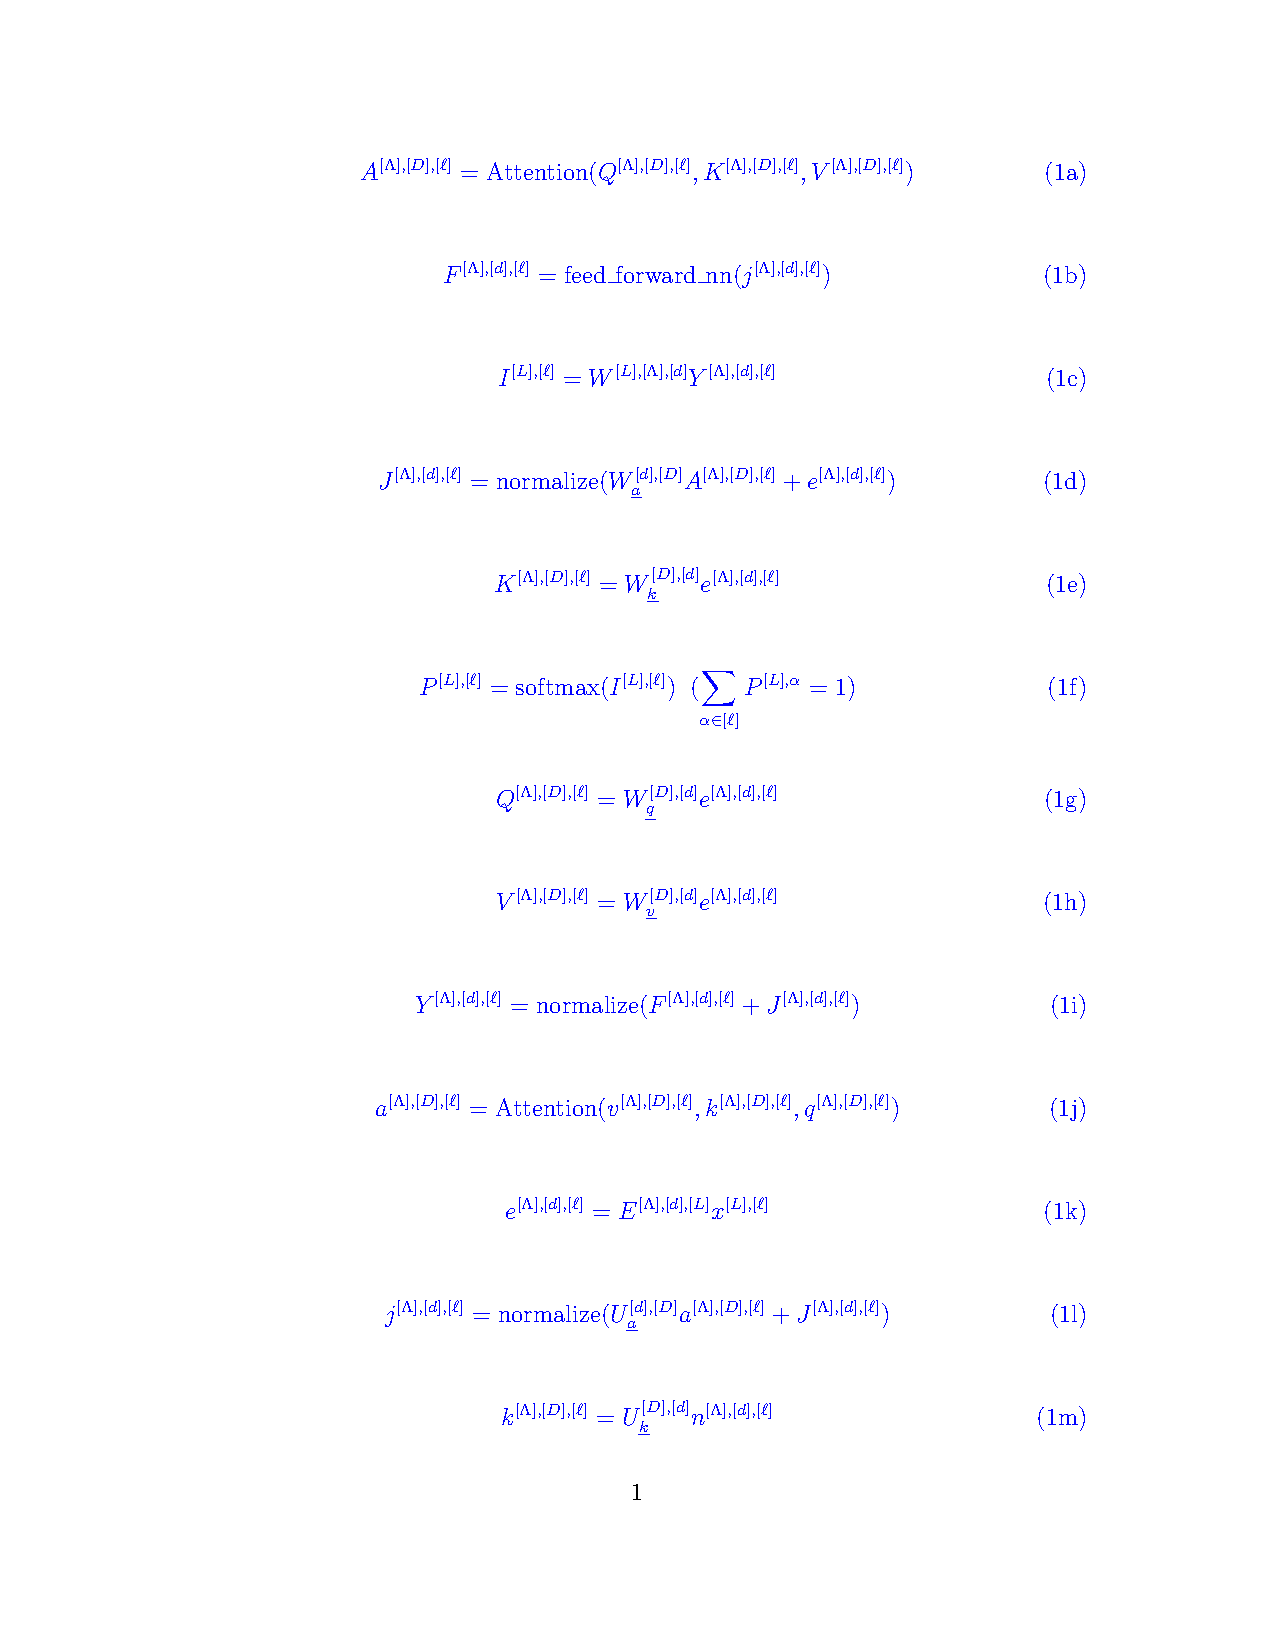
\includegraphics[width=2in]{decoder.jpg}
\end{minipage}%blank lines between minispaces breaks this
\begin{minipage}{.5\linewidth}
$$\xymatrix{
&&&*+[F*:SpringGreen]{\underline{G}^{(3, 4)}}
\\
&&&*+[F*:Orchid]{\underline{I}^{(3, 4)}}\ar[u]
\\
&&&*+[F*:yellow]{\underline{Y}^{(3, 4)}}\ar[u]
\\
&&*+[F*:SkyBlue]{\underline{B}^{(3, 4)}}\ar[ur]&
\\
&&&*+[F*:yellow]{\underline{j}^{(3, 4)}}
\\
*+[F*:Dandelion]{\underline{O}^{(3, 4)}}\ar[urrr]&&&
\\
&&&*+[F*:yellow]{\underline{a}^{(3, 4)}}\ar[uuuu]\ar[uuul]\ar[uu]\ar[ulll]
\\
&&*+[F*:Dandelion]{\underline{o}^{(3, 4)}}\ar[ur]&
\\
&*+[F*:Dandelion]{\underline{Q}^{(3, 4)}}\ar[ur]&*+[F*:Dandelion]{\underline{K}^{(3, 4)}}\ar[u]&*+[F*:Dandelion]{\underline{V}^{(3, 4)}}\ar[ul]
\\
&&&*+[F*:gray]{\underline{p}^{(3, 4)}}\ar[uuu]\ar[ull]\ar[ul]\ar[u]
\\
*+[F*:Dandelion]{\underline{q}^{(3, 4)}}\ar[uuuuu]&*+[F*:Dandelion]{\underline{v}^{(3, 4)}}\ar[uuuuul]&&*+[F*:Lavender]{\underline{R}^{(3, 4)}}\ar[u]
}$$
\end{minipage}
\caption{Decoder.}
\label{fig-texnn-for-decoder}
\end{figure}

\begin{subequations}

\begin{equation}\color{blue}
G^{(3, 4)} = I^{(3, 4)}
\label{eq-G-fun-decoder}
\end{equation}

\begin{equation}\color{blue}
I^{(3, 4)} = Y^{(3, 4)}
\label{eq-I-fun-decoder}
\end{equation}

\begin{equation}\color{blue}
Y^{(3, 4)} = B^{(3, 4)},a^{(3, 4)}
\label{eq-Y-fun-decoder}
\end{equation}

\begin{equation}\color{blue}
B^{(3, 4)} = a^{(3, 4)}
\label{eq-B-fun-decoder}
\end{equation}

\begin{equation}\color{blue}
j^{(3, 4)} = O^{(3, 4)},a^{(3, 4)}
\label{eq-j-fun-decoder}
\end{equation}

\begin{equation}\color{blue}
O^{(3, 4)} = q^{(3, 4)},v^{(3, 4)},a^{(3, 4)}
\label{eq-O-fun-decoder}
\end{equation}

\begin{equation}\color{blue}
a^{(3, 4)} = o^{(3, 4)},p^{(3, 4)}
\label{eq-a-fun-decoder}
\end{equation}

\begin{equation}\color{blue}
o^{(3, 4)} = Q^{(3, 4)},K^{(3, 4)},V^{(3, 4)}
\label{eq-o-fun-decoder}
\end{equation}

\begin{equation}\color{blue}
Q^{(3, 4)} = p^{(3, 4)}
\label{eq-Q-fun-decoder}
\end{equation}

\begin{equation}\color{blue}
K^{(3, 4)} = p^{(3, 4)}
\label{eq-K-fun-decoder}
\end{equation}

\begin{equation}\color{blue}
V^{(3, 4)} = p^{(3, 4)}
\label{eq-V-fun-decoder}
\end{equation}

\begin{equation}\color{blue}
p^{(3, 4)} = R^{(3, 4)}
\label{eq-p-fun-decoder}
\end{equation}

\begin{equation}\color{blue}
R^{(3, 4)} =
\label{eq-R-fun-decoder}
\end{equation}

\begin{equation}\color{blue}
q^{(3, 4)} =
\label{eq-q-fun-decoder}
\end{equation}

\begin{equation}\color{blue}
v^{(3, 4)} =
\label{eq-v-fun-decoder}
\end{equation}

\end{subequations}


\end{document}  
